\subsection*{Introduction}

The concept of phase permeates seismic data processing and signal processing in general, but it can be awkward to understand, and manipulating it directly can lead to surprising results. It doesn’t help that the word phase is used to mean a variety of things, depending on whether we refer to the propagating wavelet, the observed wavelet, post-stack seismic attributes, or an entire seismic data set. Several publications have discussed the concepts and ambiguities \citep{Roden1999significance, Liner2002Phase, 2002Tutorial}.



  \begin{figure}[ht]
    \centering
    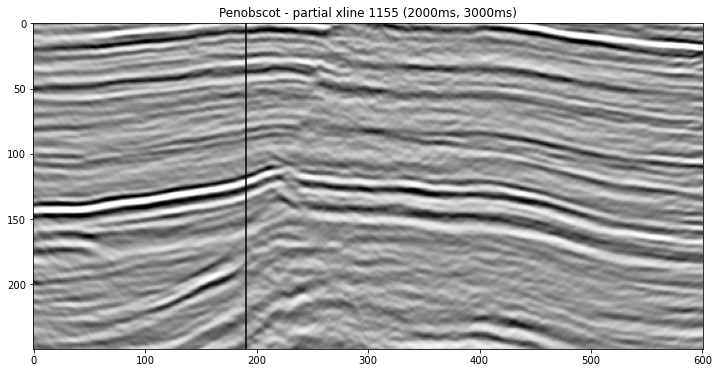
\includegraphics[width=1.0\linewidth]{images/RkW3EUemHJbWfgejvqYu_ihBcaiMuiszbc8xSI8bd.18-output-0.png}
  \end{figure}


\textit{Figure 1 - Partial seismic crossline section from the Penobscot 3D survey between 2000m - 3000m with vertical line marking the extracted trace of interest.}

The data we are using are the Penobscot 3D \citep{Purves2014Phase} survey from the Open Seismic Repository (\url{https://opendtect.org/osr/}), which is openly licensed CC-BY-SA by the Canada Nova Scotia Offshore Petroleum Board, and dGB Earth Sciences.

In this tutorial, we will focus on aspects of phase relevant to the interpreter. We will look at how to manipulate the phase of a seismic trace by manipulating the phase of its Fourier transform and will use that idea to generate the well-known instantaneous phase post-stack attribute. We will also check how close to zero phase our test data set is.

The plots included in this tutorial were created using standard python libraries and the code to reproduce them is available here on Curvenote and on the \href{https://github.com/seg/tutorials-2014/tree/master/1410_Phase}{SEG tutorials GitHub repo}.

\subsection*{The Hilbert Transform}

The Fourier transform is complex. Taking the transform of any real signal will result in a set of complex coefficients. Complex numbers are essentially 2D vectors, meaning they have two components: magnitude and phase angle. Most of the time when dealing with Fourier transforms, we concentrate on magnitude, which tells us about the distribution of signal energy through frequency. However, every signal also has a phase spectrum, and the phase encodes the signal’s structure —  the distribution of the signal energy through time. We do not often examine phase spectrum because it is difficult to interpret, but we can manipulate Fourier phase to change the structure of our signal without affecting its amplitude spectrum.

The Hilbert transform is a linear operator that produces a 90˚ phase shift in a signal, and it is a good first step in our exploration of phase. It is also commonly used in post-stack seismic analysis to generate the analytic signal from which we can compute the standard complex trace attributes such as envelope, instantaneous phase, and instantaneous frequency

The definition of the Hilbert transform is rather cryptic; it is much easier to consider in terms of its Fourier transform definition. The Hilbert transform $H$ of a signal $u$ is related to the Fourier transform $F$ like this:

\begin{equation}
  \label{a94216e5}
  F(H(u))(\omega) = \sigma_H(\omega) \cdot F(u)(\omega)
\end{equation}

where:

\begin{equation}
  \label{a26fb23d}
  \sigma_{\mathrm{H}}(\omega)=\left\{\begin{array}{l}i \text { for } \omega<0 \\ 0 \text { for } \omega=0 \\ -i \text { for } \omega>0\end{array}\right.
\end{equation}

So we apply a Hilbert transform by multiplying all negative frequencies by $i$and all positive frequencies by $-i$, leaving any DC component untouched. This is perhaps not intuitive, but we can gain some additional insight by thinking about it geometrically.

The multiplication of two complex numbers $a$ (such as a Fourier coefficient) and $b$ (such as $\sigma_H$above) can be thought of as a rotation in the complex plane. Euler’s formula helps us to see that to rotate any complex number by a specific angle a, we must multiply it by the complex number $\mathrm{e}^{i \alpha}=\cos \alpha+i \sin \alpha$.

We see that multiplication by $i$ alone, as in the equation above, is equivalent to a rotation by 90°. When we take the inverse Fourier transform, the result is a phase-shifted version of our signal.

So, we can generalize the definition of the Hilbert above to produce a phase shift to any angle, $\alpha$:

\begin{equation}
  \label{a743ceff}
  \sigma_{n}(\omega)=\left\{\begin{array}{l}\mathrm{e}^{i \alpha} \text { for } \omega<0 \\ 0 \text { for } \omega=0 \\ \mathrm{e}^{-i \alpha} \text { for } \omega>0\end{array}\right.
\end{equation}

\subsection*{Phase shifting in Python 🐍}

Let us use this principle to phase-shift a seismic trace using open source python💪.

\begin{aside}
  NOTE: If you are working in GNU Octave check back to \href{https://github.com/seg/tutorials-2014/blob/master/1410_Phase/fftshifter.m}{\textit{fftshifter.m}} on github.
\end{aside}

We will take the fast Fourier transform (FFT) of our signal, manipulate the coefficients, and apply the inverse FFT.

\begin{code}[python]
from math import ceil,exp
from scipy.fftpack import fft, ifft

def fftshifter(x, phase_shift_in_radians):
    # Create an array to apply the coefficient to
    # positive and negative frequencies appropriately
    N = len(x);
    R0 = np.exp(-1j*phase_shift_in_radians);
    R = np.ones(x.shape, dtype=np.complex);
    R[0]=0.;
    R[1:N//2] = R0;
    R[N//2:] = np.conj(R0);

    # Apply the phase shift in the frequency domain
    Xshifted = R*fft(x);

    # Recover the shifted time domain signal
    y = np.real(ifft(Xshifted));

    return y
\end{code}

\subsection*{Complex Trace Attributes}

Now that we have this ability to phase-shift, what can we do with it?

We can compute some seismic attributes. A whole set of commonly used attributes depends on the Hilbert transform and the code below generates the Hilbert transform, envelope, and phase traces for a trace from the Penobscot data set.

\begin{aside}
  If you look closely here you’ll see we’re actually using the \texttt{hilbert} function from \texttt{scipy.signal} instead of our arbitrary phase shifter. Whilst the two should be equivalent for 90 degree shifts, I’ve noted that the \texttt{scipy} version is slightly different and produces smoother envelope responses, which I believe are more correct. I think this is down to a windowing step on computation of the FFT tht we are omitting in \texttt{fftshifter}, but I’ll need to check the \texttt{scipy} implementation to confirm. Stay tuned for updates on that over in the \href{https://iooxa.com/@stevejpurves/geoscience/phaseandhilbert}{notebook}.
\end{aside}

\begin{code}[python]
from scipy.signal import hilbert as hilbert_transform
hilbert = np.zeros_like(seismic)

for x in range(line.shape[0]):
    hilbert[x,:] = np.imag(hilbert_transform(line[x,:])[500:750])

z = seismic + 1j*hilbert
env = np.abs(z)
phase = np.angle(z)
\end{code}

See the accompanying notebook for full plotting code.

A section of this trace is shown in Figure 2 below.



\begin{verbatim}(2000.0, 3000.0)\end{verbatim}

  \begin{figure}[ht]
    \centering
    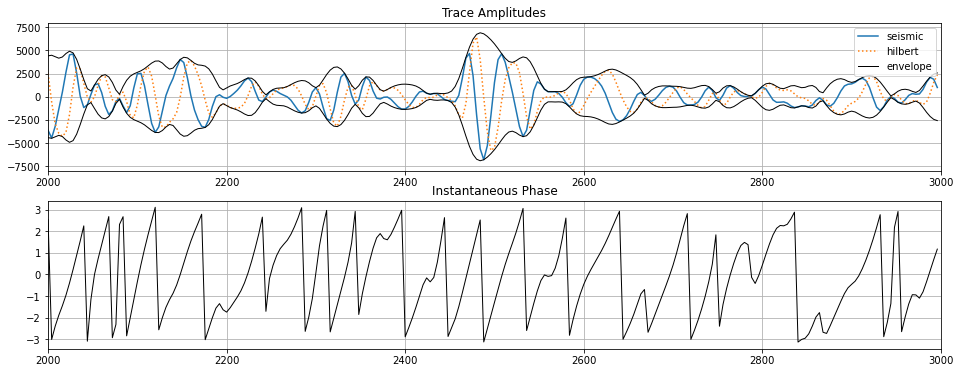
\includegraphics[width=1.0\textwidth]{images/RkW3EUemHJbWfgejvqYu_VcYeNrFMSYtf8Nu8DrSv.1-output-0.png}
  \end{figure}


\textit{Figure 2 - Single seismic trace extracted at the location marked in Figure 1. The original trace is shown in blue (top) along with the Hilbert Transform trace (orange, dashed) and Envelope function (black). The unwrapped instantaneous phase signal is also shown (bottom).}



  \begin{figure}[ht]
    \centering
    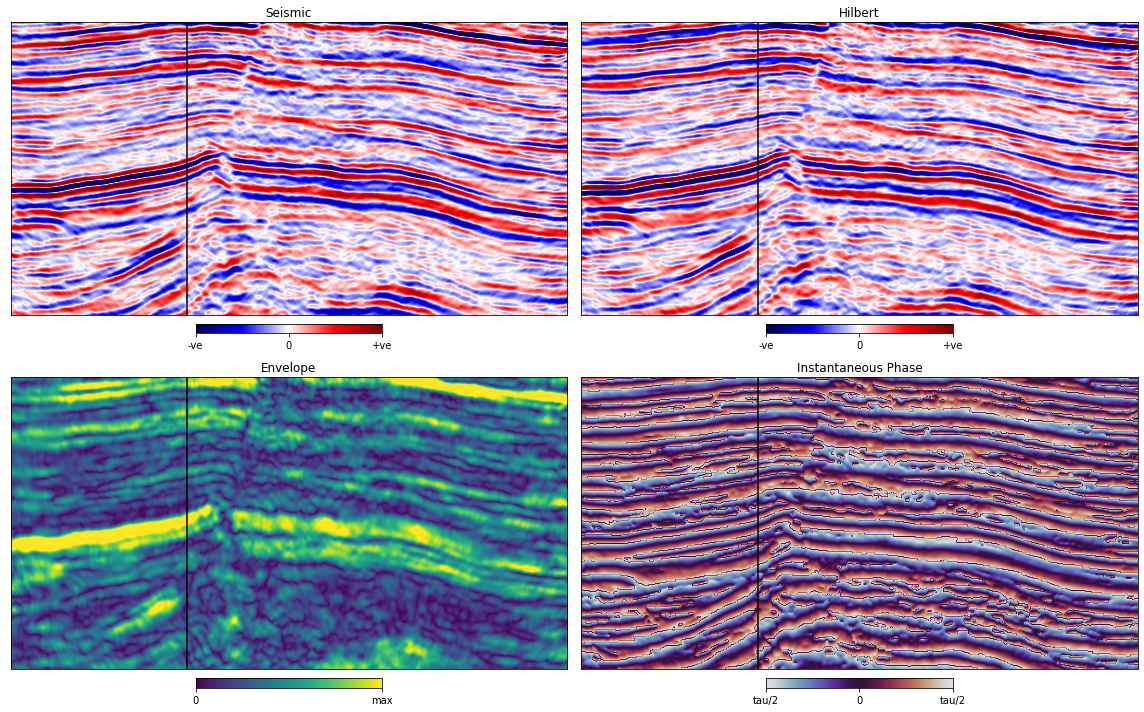
\includegraphics[width=1.0\textwidth]{images/RkW3EUemHJbWfgejvqYu_1UA1dMMyGLBD6TXFEQQP.1-output-0.png}
  \end{figure}


\textit{Figure 3 - shows the same attributes now computed over the whole section. These are useful interpretation aids.}

Once you have the complex trace representation, z, there are many additional attributes that you can compute, such as instantaneous frequency, phase acceleration, and envelope-weighted frequency, the list goes on… merely by playing around with the complex trace.

\subsection*{Checking the phase of your seismic}

The complex attributes generated from a seismic trace and its Hilbert transform are useful in seismic interpretation. However, the quality of our seismic interpretation depends on another aspect of phase, that is, the phase of our seismic data set and whether the observed wavelet has been corrected to a zero-phase response during processing. Roden and Sepúlveda (1999) give a practical way to assess the phase of seismic data as a quality check for seismic interpretation. They point out that where we have a strong reflection from a sharp geologic interface that we can confidently expect to produce a zero-phase response, we can measure the actual response in the seismic data set on that horizon to determine the amount of phase error present. The principle that Roden and Sepúlveda (1999) apply is that at strong reflections in zero phase data, we would expect peaks (or troughs) in the trace to align with peaks in the envelope. Therefore, any horizon that we pick on zero-phase data could also be picked on the envelope of that data.

Figure 4 shows a segment of our trace from Figure 1 with envelope peaks marked as spikes (see find\_peaks.m). In Figure 2b, I have isolated those events and plotted the actual signal phase against the phase we would expect for a zero-phase data set.

The difference between the two could be systematic residual phase. If we think a particular reflector has minimal interference and no AVO or other effects, then the rest is residual phase. The strong trough at the Abenaki reflector in Figure suggests that there could be 0.64 radians, or about 37°, of residual phase in the data. That is something that we could now correct for by phase-shifting all our traces.



  \begin{figure}[ht]
    \centering
    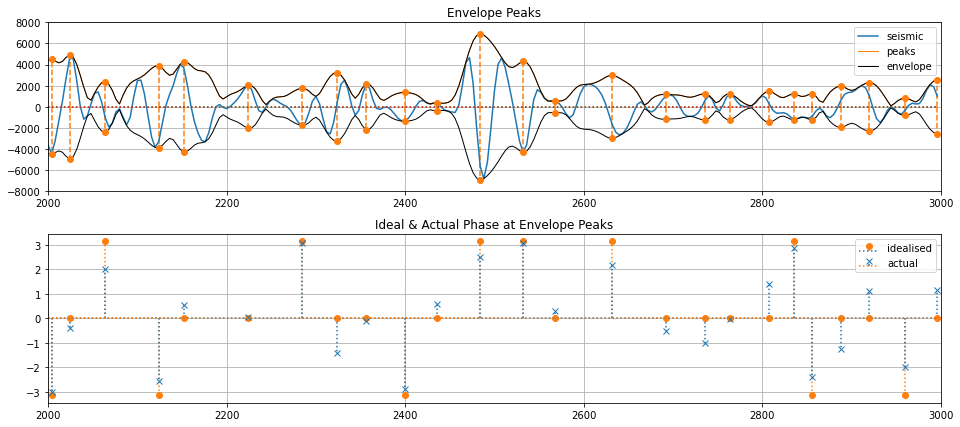
\includegraphics[width=1.0\textwidth]{images/RkW3EUemHJbWfgejvqYu_tIrSeE4eYvSa9LqwFLrq.1-output-0.png}
  \end{figure}


\textit{Figure 4 - (top) The trace previously shown in Figure 1, with envelope peaks marked as impulses. (bottom) the idealized and actual phase of the signal at each envelope peak. Phase errors at strong envelope peaks are initiators of residual phase error in our data.}

We can also look at this phase error at envelope peaks across our dataset as shown in Figure 5 below.



  \begin{figure}[ht]
    \centering
    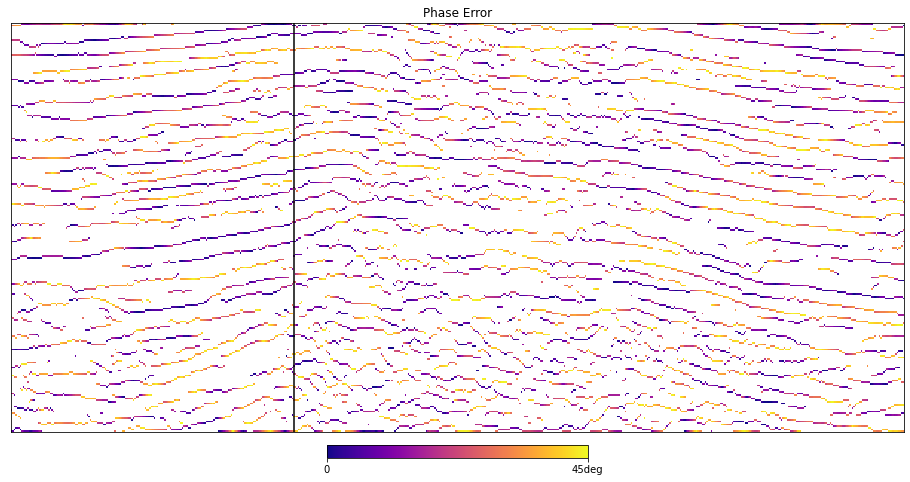
\includegraphics[width=1.0\textwidth]{images/RkW3EUemHJbWfgejvqYu_nntW22fEZdfrz19UE7Ma.1-output-0.png}
  \end{figure}


\textit{Figure 5 - phase error computed at peaks of the Envelope function on each trace.}

The Hilbert transform opens up a world of seismic attributes, some of which have everyday application for the interpreter. To run or build on the code clone the repo at \url{http://github.com/seg/tutorials-2014}.

\subsection*{Acknowledgements}

The official version of this tutorial was published in the SEG’s Leading Edge Magazine in October 2014.


\begin{center}
  
\includegraphics[width=0.2\linewidth]{images/RkW3EUemHJbWfgejvqYu_vLdgP59PLnWWrXcZOjTv.1.jpg}
\end{center}
The tutorial is Open Access and licensed under \href{https://creativecommons.org/licenses/by-sa/4.0/}{Creative Commons Share-Alike 4.0 (CC-BY-SA 4.0)}.

\begin{callout}
  The official tutorial can be found here: \url{https://doi.org/10.1190/tle33101164.1}

  The SEG GitHub repo for the tutorials is here: \url{https://github.com/seg/tutorials-2014}
\end{callout}

This article is a refresh of the original that uses python in place of GNU Octave. It includes all of the figures from the original pre-publication draft. This article is also licensed under \href{https://creativecommons.org/licenses/by-sa/4.0/}{CC-BY-SA 4.0}.

The full code is available in \href{https://curvenote.com/blocks/RkW3EUemHJbWfgejvqYu/mNnJgVOim6kyzo1p5ipL}{phase\_and\_hilbert\_transform.ipynb}

